\documentclass[letterpaper,twocolumn,amsmath,amsfont,amssymb,english,aps,jcp,preprintnumbers,groupaddress,nofootinbib,tightenlines]{revtex4}

\usepackage{graphicx}
\usepackage{epstopdf}

%\documentclass[aps,prb,letterpaper,twocolumn,nofootinbib,showkeys]{revtex4-1}
%\documentclass[aps,amssymb,prl,letterpaper,twocolumn,nofootinbib,showkeys]{revtex4-1}

%\usepackage[backend=bibtex]{biblatex}

%    backend=biber,
%    style=authoryear,
%    natbib=true,
%    sortlocale=en_US,
%    url=false,
%    doi=true,f
%    eprint=false
%]{biblatex}
%\usepackage{hyperref}


\newcommand{\mat}[1]{\boldsymbol{#1}}
\newcommand{\mmat}[1]{\widetilde{\boldsymbol{#1}}}
\newcommand{\matT}[1]{\boldsymbol{#1}^\dagger}
\newcommand{\ot}{ {\scriptstyle \otimes}_{ \tau } }

%%\hypersetup{pdftitle={FreeON Project Report 1}}
%\hypersetup{pdfauthor={Matt Challacombe and Nicolas Bock}}
%\hypersetup{pdfsubject={A SpAMM Stabilized Newton Schulz Preconditioner: Fighting Error with Error}}

%\bibstyle{aipnum4-1}

\begin{document}

\title{On Stability of Newton Schulz Iterations in an Approximate Algebra}

\author{Matt Challacombe}
\email{matt.challacombe@freeon.org}
\homepage{http://www.freeon.org}
\affiliation{Theoretical Division, Los Alamos National Laboratory}

\author{Nicolas Bock}
\email{nicolasbock@freeon.org}
\homepage{http://www.freeon.org}
\affiliation{Theoretical Division, Los Alamos National Laboratory}

%\begin{abstract}
%Forward look
%\end{abstract}

\maketitle
\section{Introduction}

In many areas of application, finite correlations lead to matrices with decay properties.  By decay, we mean an approximate 
(perhaps bounded \cite{}) inverse relationship between matrix elements and an associated distance;  this may be a simple inverse 
exponential relationship between elements and the Cartesian distance between support functions, or it may 
involve a generalized distance, {\em e.g.}~ a statistical measure between strings.  
In electronic structure,  correlations manifest in decay properties of the gap shifted matrix 
sign function, as projector of the effective Hamiltonian (Fig.~\ref{figure1}).  
More broadly, matrix decay properties may coorespond to statistical matrices 
\cite{penrose1974,voit00,Anselin2003,Hardin2013,Krishtal2014}, including learned correlations in a 
generalized, non-orthogonal metric \cite{}. More broadly still, problems with local, non-orothogonal support 
are often solved with congruential transformations of the matrix inverse square root \cite{Lowdin56,naidu11} or a related factorization \cite{Krishtal2014};
these transformations correlate local support with a representation independent form, {\em eg.}~of the eigenproblem. 
Interestingly, the matrix sign function and the matrix inverse square root function are related by Higham's identity:
\begin{equation}
\rm{sign} \left( \begin{bmatrix} 0 & \mat{s}      \\ \mat{I}       & 0\end{bmatrix} \right)  =
                 \begin{bmatrix} 0 & \mat{s}^{1/2} \\ \mat{s}^{-1/2} & 0\end{bmatrix}  .
\end{equation}
A complete overivew of matrix function theory and computation is given in Higham's enjoyable reference \cite{Higham08}. 

A well conditioned matrix $\mat{s}$ may often correspond to matrix sign and inverse square root functions with rapid exponential decay, 
and be amenable to the sparse matrix approximation
$\bar{\mat{s}} = \mat{s}+ \mat{\epsilon}^{\mat{s}}_\tau$, where $\mat{\epsilon}^{\mat{s}}_\tau$ is the error introduced according to some  
criteria $\tau$.  Supporting this approximation are usefull bounds to matrix function elements \cite{Benzi99b, }.  
The criteria $\tau$ might be a drop-tolerence, 
$\epsilon^{\mat{s}}_{\tau} = \{-s_{ij}*\hat{\mat{e}}_i \, | \, |s_{ij}|<\tau \}$, a radial cutoff, 
$\epsilon^{\mat{s}}_{\tau} = \{-s_{ij}*\hat{\mat{e}}_i \, | \, \lVert \mat{r}_i - \mat{r}_j \rVert > \tau \}$, 
or some other approach to truncation, perhaps involving a sparsity pattern chosen {\em a priori}. 
Then, conventional computational kernels may be employed, such as the sparse general matrix-matrix multiply 
($\tt{SpGEMM}$) \cite{Gustavson78, Toledo97,challacombe00,bowler00}, yeiding fast solutions for multiplication rich iterations and a modulated fill in. 
These and related incomplete/inexact approaches to the computation of sparse approximate matrix functions often lead to ${\cal O}(n)$ 
algorithms, finding wide use in technologically important preconditioning schemes, the information sciences, electronic structure and many
other disciplines.  Comprehensive surveys of these methods in the numerical linear algebra are given by Benzi \cite{Benzi99,Benzi02}, and
by Bowler \cite{Bowler12} and Benzi \cite{Benzi13} for electronic structure.

\begin{figure}[t]\label{figure1}
 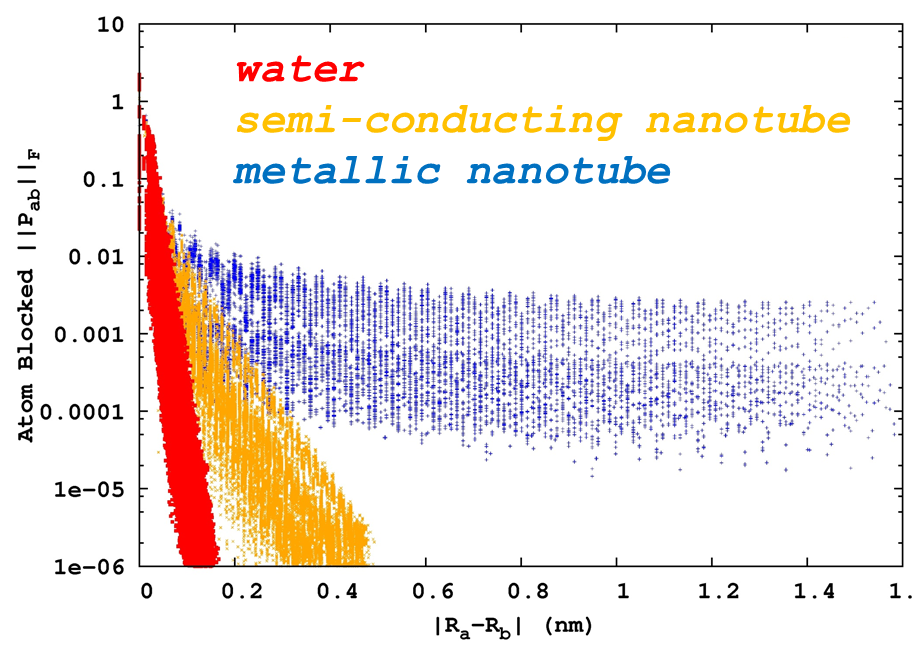
\includegraphics[width=3.5in]{decay_picture.png}
  \caption{Examples from electronic structure of decay for the spectral projector (gap shifted sign function) with respect to local (atomic) support.  
           Shown is decay for systems with correlations that are short (insulating water), medium (semi-conducting 4,3 nanotube), and 
           long (metalic 3,3 nanotube) ranged,  from exponential (insulating) to algebraic (metallic). }
\end{figure}

Because the truncated multiplication is controled only by absolute, addititve errors in the  product,   
\begin{equation}
\overline{ \mat{a} \cdot \mat{b} }\; = \; \mat{a}\cdot\mat{b} \; +\; \mat{\epsilon}^{\mat{a}}_\tau \cdot \mat{b} \;+\;
 \mat{a} \cdot \mat{\epsilon}^{\mat{b}}_\tau  \; + \;   {\mathcal O}(\tau^2)
\end{equation}
achieving sparse, stable and rapidly convergent iteration for ill-conditioned problems can be challenging \cite{}.  In cases of 
extreme degeneracy,  hierarchical semi-seperable (reduced rank) algorithms  can offer effective complexity reduction \cite{}.
However, many pratical cases are somewhere in-between sparse and meaningfully degenerate regimes; effectively dense but without
an exploitable reduction in rank.  This is the case in electronic structure for strong but non-metalic correlation, 
{\em e.g.}~towards the Mott transition \cite{}, and also in the case of local atomic support towards completeness \cite{Others, Hutter, Gigi}. 

\pagebreak
In this contribution, we consider an $N$-body approach to the approximation of matrix functions with decay, 
based on the quadtree data structure \cite{wise, samet} 
\begin{equation}
\mat{a}^i = \begin{bmatrix} \,  \mat{a}^{i+1}_{00} \, & \,  \mat{a}^{i+1}_{01} \,  \\[0.2cm]  \, \mat{a}^{i+1}_{10} \,  & \,\mat{a}^{i+1}_{11} \, \end{bmatrix} \, ,
\end{equation}
and orderings that are locality preserving \cite{}.  Orderings that preserve data locality are well developed in the
database theory \cite{}, providing fast spatial and metric querries.  
Locality enabled, fast data access is central to the $N$-Body approximation \cite{}, and an important problem 
for enterprise \cite{} and runtime systems \cite{}, with memory hierarchies becoming increasingly assynchronous and decentralized \cite{cache}.  
For matrices with decay, orderings that preserve locality lead to block-by-magnitude matrix structures with well 
segregated neighborhoods, inhabited by matrix elements of like size, and efficiently resolved by the quadtree data structure \cite{}.

With block-by-magnitude ordering of matrices $\mat{a}$ and $\mat{b}$, 
the Sparse Approximate Matrix Multiplication ($\tt SpAMM$) kernel,  $\ot$, carries out fast 
occlusion culling of insignifcant volumes in the product octree:
\begin{widetext}
\begin{equation}
\mat{a}^{i} \ot \mat{b}^{i} = 
\left\{
        \begin{array}{ll}
                 \emptyset \quad \tt{if}\quad \lVert \mat{a}^i \rVert \lVert \mat{b}^i \rVert < \tau \\[0.2cm]
                 \mat{a} ^i \cdot \mat{b}^i \quad  \tt{if}(i=\tt{leaf}) \\[0.2cm]
\begin{bmatrix} \mat{a}^{i+1}_{00} \ot \mat{b}^{i+1}_{00} +\mat{a}^{i+1}_{01} \ot \mat{b}^{i+1}_{10} \; , \; &
                \mat{a}^{i+1}_{00} \ot \mat{b}^{i+1}_{01} +\mat{a}^{i+1}_{01} \ot \mat{b}^{i+1}_{11}  \\[0.2cm] 
                \mat{a}^{i+1}_{00} \ot \mat{b}^{i+1}_{01} +\mat{a}^{i+1}_{01} \ot \mat{b}^{i+1}_{11} \; , \; & 
                \mat{a}^{i+1}_{00} \ot \mat{b}^{i+1}_{01} +\mat{a}^{i+1}_{01} \ot \mat{b}^{i+1}_{11}   
\end{bmatrix}  \quad \tt{else}
                \end{array}
              \right.  \, ,
\end{equation}
\end{widetext}
with errors bounded by sub-multiplicative norms, $\lVert \cdot \rVert \equiv \lVert \cdot \rVert_F$, and the Cauchy-Schwarz inequality \cite{kahan}.
The $\tt SpAMM$ error 
\begin{equation}
\mat{\Delta}^{a\cdot b}_{\tau}=\mat{a} \ot \mat{b}-\mat{a}\cdot \mat{b} 
\end{equation}
corresponds to an occlusion volume in the product space,  obeying the multiplicative bound 
\begin{equation}
\lVert \mat{\Delta}^{a \cdot b}_{\tau} \rVert \, \leq \, \tau \, \lVert \mat{a} \rVert  \,  \lVert \mat{b} \rVert \, .
\end{equation}
The $\tt SpAMM$ kernel is {\em fast} and {\em stable} in the Demmel, Dumitriu and Holz sense \cite{Demmel07}, enabling
a {\em relative} error control in the product.  Unlike roundoff error however, the $\tt SpAMM$ error is deterministic,
leading to a non-associative algebra and the development of error flows associated with the Lie bracket
\begin{equation}
\left[ \mat{a} , \mat{b} \right]_{\tau} = \mat{a} \ot \mat{b}-\mat{b} \ot \mat{a}  
=  \left[ \mat{a} , \mat{b} \right]
+ \mat{\Delta}^{a\cdot b}_{\tau} -\mat{\Delta}^{b\cdot a}_{\tau} \,.
\end{equation}
$\tt SpAMM$ is similar to compressed sensing kernels for sketching the matrix product \cite{Kutzkov2012, Pagh2013}.  Instead of
the FFT however, compression is achieved simply through fast metric querry of the occlusion map, which may expreience 
localiztion effects in the basin of stability.   In addition to complexity reduction, octree locality is 
important for the communication optimality of $N$-body methods \cite{}.   This $n-$body approach is 
diemtric to randomization techniques that employ homogenization to well condition matrices 
\cite{pan, DiahLi and Parket Scott},  and also for distributed memory implementations of the $\tt SpGEMM$ \cite{}.

\section{First Order Newton-Shulz Iteration}

The approximation of the matrix sign and inverse square root via first order Newton Schulz (NS) iteration 
has a number of attractive features, notably multiplication richness and quadratic convergence in the basin of convergence. 
Developed extensively by Higham \cite{}, NS  yeilds resolution of the identity through the square root and its inverse \cite{}:
\begin{equation}
sign \left( \mat{s} \right) =\mat{s}^{1/2} \cdot \mat{s^{-1/2}} \, .
\end{equation}
positive definate argument $\mat{s}$, and stability of the iteration as the residual $\mat{x}_k $ tends towards 
idempotence, $\mat{x}_k \rightarrow {sign}\left( \mat{s} \right) $, with 
 $\mat{y}_k \rightarrow \mat{s}^{1/2}$  and $\mat{z}_k \rightarrow \mat{s}^{-1/2}$ \cite{higham}. 
Convergence and stability are determined by the first order NS map $m[\mat{x}]=\frac{\sqrt{\alpha}}{2} \left(3-\alpha \mat{x} \right)$, 
with scaling $\alpha$ \cite{}. 
Initially, $m'$ at the smallest eigenvalue $x_0$ controls the rate of progress towards idempotence.  
Later, the overall eigenvalue distribution becomes important \cite{}. Pan and Scriber .  More recently, 
Jie and Chen demonstrated a factor of two reduction 
in the number of NS steps for ill-conditioned problems by chosing $\alpha \sim 2.85$, with damping towards $\alpha=1$ at 
convergence.  

First order NS iteration converges linearly towards a basin of stability, marked by super-linear convergence 
and associated with sign iteration,  $\mat{x}_k \leftarrow sign \left( \mat{x}_{k-1} \right)$. 
Bai and Demmel \cite{}, Byers, He and Mehrmann \cite{} and Higham (Ref.\cite{} Section 5.7)
show that within this basin, commuting errors $\mat{x}_k+\delta \mat{x}_k$ \cite{}  
are anihilated to first order, depending on the differential $\delta \mat{x}_k < 1 $. 
Ideally, a $\tau$ can be found yeilding fast computation with precision sufficient to gain the basin of stability.  From the
preconditioned state then, additional corrections can be made to the residual at little additional 
cost, allowing the eigenvector basis of the argument to be kept tightly 
\footnote{Sometimes refered to as the ``variational'' property of early ``spectral projection as optimization'' 
techniques, with gradients based on the argumental eigenvectors \cite{}.}

However, NS iteration can diverge due to the unbounded accumulation of errors ($\delta \mat{x}_k > 1 $).
For ill-conditioned problems, and with an approximate non-commuting algebra, the stability properties of various NS 
forms can be very different,  depending on the {\em handedness} of opperations and their proximity to the argument $\mat{s}$.
Starting with $\mat{z}_0=\mat{I}$ and $\mat{x}_0=\mat{y}_0=\mat{s}$, these nominally equivalent forms include: the ``dual'' iteration,
\begin{eqnarray}
\mmat{y}^{\tt d}_{k}  &\leftarrow& m \left( \mmat{x}^{\tt d}_{k-1} \right) \; \ot \;  \mmat{y}^{\tt d}_{k-1}  \\
\mmat{z}^{\tt d}_{k}  &\leftarrow& \mmat{z}^{\tt d}_{k-1}  \; \ot \;  m \left( \mat{x}^{\tt d}_{k-1} \right) \\
\mmat{x}^{\tt d}_{k} &\leftarrow& \mmat{y}^{\tt d}_{k} \; \ot \; \mmat{z}^{\tt d}_{k} \; ,
\end{eqnarray}
the ``naive'' iteration,
\begin{eqnarray}
\mmat{z}^{\tt n}_{k}  &\leftarrow& \mmat{z}^{\tt }_{k-1} \; \ot \; m \left( \mmat{x}^{\tt n}_{k-1} \right) \\
\mmat{x}^{\tt n}_{k} &\leftarrow& \mmat{z}^{\tt n}_{k} \; \ot \; \mat{s} \; \ot \; \mmat{z}^{\tt n}_{k} \; ,
\end{eqnarray}
and the ``stablized'' iteration,
\begin{eqnarray}
\mmat{z}^{\tt s}_{k}  &\leftarrow& \mmat{z}^{\tt s}_{k-1}  \; \ot \; m \left( \mmat{x}^{\tt s}_{k-1} \right) \\
\mmat{x}^{\tt s}_{k} &\leftarrow& \mmat{z}^{\tt s \, \dagger}_{k} \; \ot \; \mat{s} \; \ot \; \mmat{z}^{\tt s}_{k} \; .
\end{eqnarray}


$\delta  \mat{x}}_k = \widetilde{\mat{x}}_k - \mat{x}_k $  



% For well conditioned problems, incomplete/inexact approximations 
% and the $\tt SpGEMM$ kernel offer fast solutions \cite{}.  For ill-conditioned problems however, fill in remains a 
% challenge \cite{}, showing up well before matrix-compression technologies become effective.   
% In this contribution, we develop the $\tt SpAMM$ kernel for NS iteration at index $k$, focusing on eigenvector (basis) fidelity to the



Analyses of these iterations is challenging, because of accumulated and accumulating errors with each mapping $\ot$, 
and because the errors are non-commutative.  We model each NS iteration as a multi-channel process of error accumulation, 
were for example 
\begin{eqnarray}
\widetilde{\mat{x}}^{\tt s}_k &=& f^{\tt s} \left[\widetilde{\mat{z}}_{k-1} , \widetilde{\mat{x}}_{k-1} \right] \\ 
&=&
\tt{m} \left[ \widetilde{\mat{x}}_{k-1}\right] \cdot \widetilde{\mat{z}}^\dagger_{k-1}  
\cdot \mat{s} \cdot \widetilde{\mat{z}}_{k-1} \cdot \tt{m}\left[ \widetilde{\mat{x}}_{k-1} \right] 
\nonumber
\end{eqnarray}

\begin{equation}
\delta \mat{x}_k = {f}_{\delta \mat{z}_{k-1}}  \, \lVert \delta \mat{z}_{k-1} \rVert 
                              +  {f}_{\delta \mat{x}_{k-1}}   \, \lVert \delta \mat{x}_{k-1} \rVert 
                                                                                      + {\cal{O}} \left(  \tau^2 \right)
\end{equation}





\begin{equation}
\delta \mat{x}^{\rm{naiv}}_k =   \delta  \widetilde{ \mat{z}}_{k} \cdot \mat{s} \cdot \widetilde{\mat{z}}_{k} 
                           +  \widetilde{\mat{z}}_{k} \cdot \mat{s} \cdot \! \delta \widetilde{\mat{z}}_{k} 
\end{equation}



\begin{equation}
\delta \mat{x}^{\rm{dual}}_k =   \delta  \widetilde{ \mat{y}}_{k} \cdot \widehat{\mat{z}}_{k} 
                           +  \widetilde{\mat{y}}_{k} \cdot \delta \widetilde{\mat{z}}_{k} 
\end{equation}



generalized Gateaux differential

\begin{eqnarray}
f_{\delta \mat{z}_{k-1}} &=& \lim_{\tau \rightarrow 0} \frac{ f [ \mat{z}_{k-1} +\tau  \delta \widehat{\mat{z}}_{k-1}, \widetilde{\mat{x}}_{k-1} ]
-f [\, \mat{z}_{k-1}, \widetilde{\mat{x}}_{k-1} ]  }{\tau} \nonumber  \\[0.1cm] 
&=&{L}_{\widetilde{\mat{x}}_k}\left(\widetilde{\mat{z}}_{k} , \delta \widehat{\mat{z}}_{k-1} \right)  
\end{eqnarray}

\begin{eqnarray}
f_{\delta \mat{x}_{k-1}} &=& \lim_{\tau \rightarrow 0} \frac{ f [ \widetilde{\mat{z}}_{k-1}, \mat{x}_{k-1} + \tau \delta \widehat{\mat{x}}_{k-1} ]
-f [ \widetilde{\mat{z}}_{k-1}, \mat{x}_{k-1} ]  }{\tau} \nonumber  \\[0.1cm] 
&=&{L}_{\widetilde{\mat{x}}_k}\left(\widetilde{\mat{z}}_{k} , \delta \widehat{\mat{x}}_{k-1} \right)  
\end{eqnarray}

\begin{multline}
{L}_{\widetilde{\mat{x}}_k}\left(\widetilde{\mat{z}}_{k} , \delta \widehat{\mat{x}}_{k-1} \right) 
= \delta \widehat{\mat{x}}^\dagger_{k-1} \cdot   \tt{m}'\left[\mat{x}_{k-1} \right] \cdot 
\{\widetilde{\mat{z}}^\dagger_{k-1}  \cdot \mat{s} \cdot \widetilde{\mat{z}}_{k} \}  \\
+ \{ \widetilde{\mat{z}}^\dagger_{k} \cdot \mat{s} \cdot  \widetilde{\mat{z}}_{k-1} \} 
\cdot \tt{m}'\left[\mat{x}_{k-1} \right]  \cdot \delta \widehat{\mat{x}}_{k-1} 
\end{multline}

\begin{multline}
{L}_{\widetilde{\mat{x}}_k}\left(\widetilde{\mat{z}}_{k} , \delta \widehat{\mat{z}}_{k-1} \right) = 
\{ \tt{m}\left[\mat{x}_{k-1} \right]  \cdot \delta {\widehat{\mat{z}}}^\dagger_{k-1} 
 \cdot \mat{s} \} \cdot \widetilde{\mat{z}}_{k} \\
+\widetilde{\mat{z}}^\dagger_{k} \cdot \{ \mat{s} \cdot \delta {\widehat{\mat{z}}}_{k-1}
\cdot \tt{m}\left[\mat{x}_{k-1} \right]    \} 
\end{multline}

\begin{equation}
 \{ \widetilde{\mat{z}}^\dagger_{k} \cdot \mat{s} \cdot  \widetilde{\mat{z}}_{k-1} \} 
\rightarrow \mat{p}_+\left[\mat{s} \right]
\end{equation}

\begin{equation}
\{ \mat{s} \cdot \delta {\widehat{\mat{z}}}_{k-1}
\cdot \tt{m}\left[\mat{x}_{k-1} \right]    \} 
\rightarrow \mat{n}\left[\mat{s} \right]
\end{equation}

\section{Implementation}

\subsection{Methods}
FP, F08, OpenMP 4.0

\subsection{A Modified NS Map}

\subsection{$\delta \mat{x}_k$ and $\delta \mat{x}_k$ channels}
tau= Figure showing channels etc.  

\subsection{Convergence}
Map switching and etc based on TrX


\section{Ill-Conditioned Support}

\subsection{ 3,3 carbon nanotube with diffuse $sp$-function}
double exponential (Fig.)

\subsection{Water with triple zeta and double polarization}
Here's looking at you Jurg...

\section{Experiments}

\subsection{Occlusion Error Flows}
\begin{figure}[h]
  \caption{equation...}
 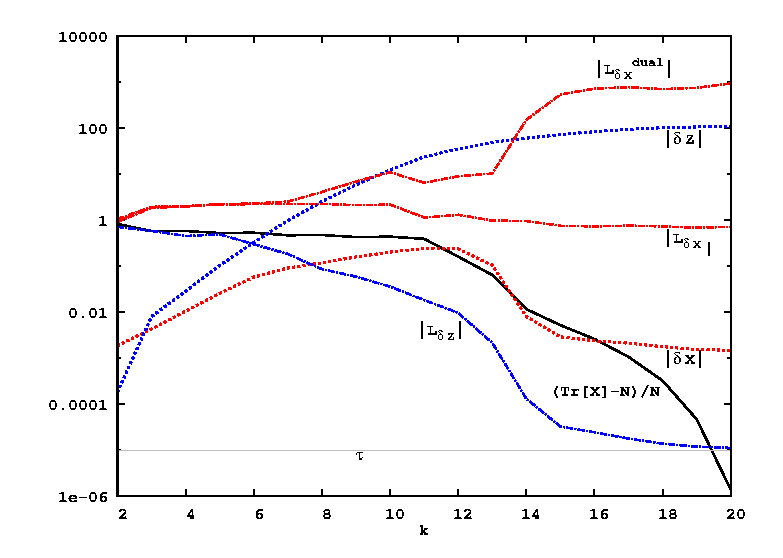
\includegraphics[width=3.5in]{8x_33_nanotube_cond10_tau-5.eps}
 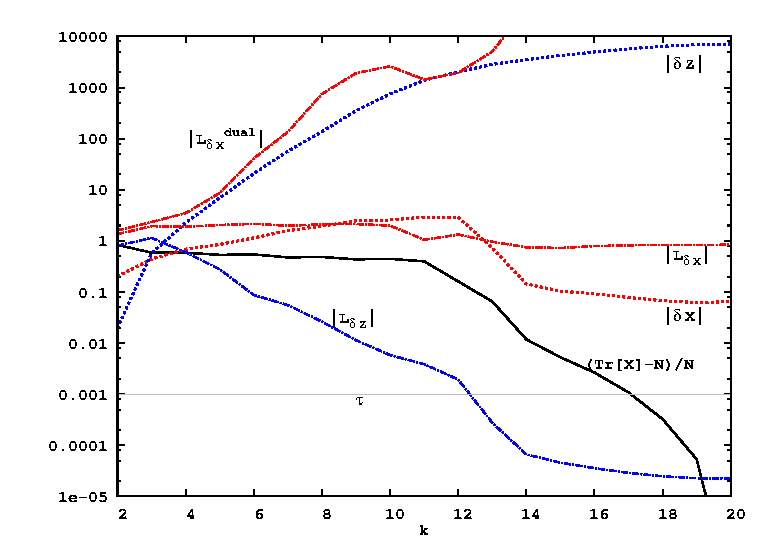
\includegraphics[width=3.5in]{8x_33_nanotube_cond10_tau-3.eps}
\end{figure}
\begin{figure}[h]
  \caption{equation...}
 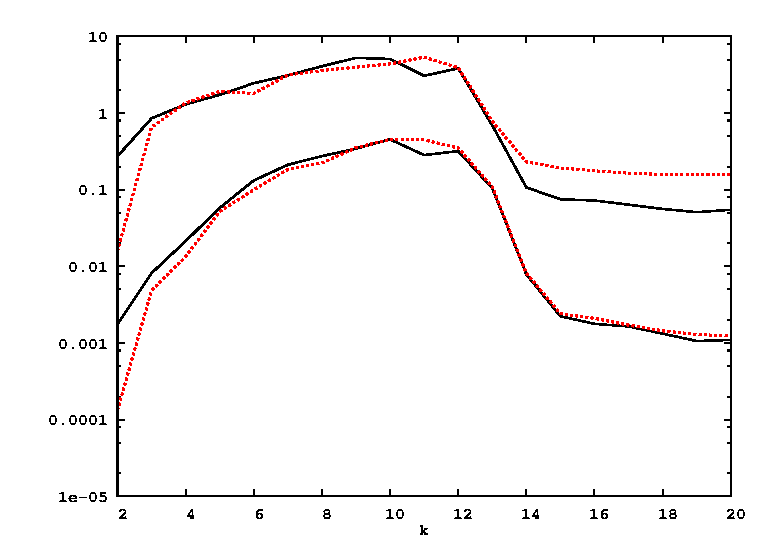
\includegraphics[width=3.5in]{8x_33_nanotube_cond10_compare_errors.eps}
\end{figure}

\subsection{Comments}

\begin{multline}
 \delta {\mat{z}}_{k-1} \approx \Delta^{\widetilde{\mat{z}}_{k-2} \cdot \tt{m}\left[ \widetilde{\mat{x}}_{k-2}\right]}_\tau 
+ \mat{z}_{k-2} \cdot \tt{m}'\left[ \widetilde{\mat{x}}_{k-2}\right] \cdot \delta \mat{x}_{k-2} \\
+\delta \mat{z}_{k-2} \cdot \tt{m} \left[\widetilde{\mat{x}}_{k-2} \right] 
\end{multline}

\begin{multline}
\lVert \delta {\mat{z}}_{k-1} \rVert \lesssim
\lVert \mat{z}_{k-2} \rVert \left( \;  \tau \, \lVert \tt{m} \left[\widetilde{\mat{x}}_{k-2} \right]  \rVert \right.   \\ \left.
+ \; \lVert \delta {\mat{x}}_{k-2} \rVert   \lVert \tt{m}' \left[\widetilde{\mat{x}}_{k-2} \right] \rVert \; \right)
\end{multline}

\begin{equation}
\lVert \mat{z}_{k} \rVert  \rightarrow \sqrt{\kappa\left(\mat{s} \right)}
\end{equation}

\subsection{Querry Surfaces}

\begin{figure}[h]
  \caption{equation...}
\fbox{ 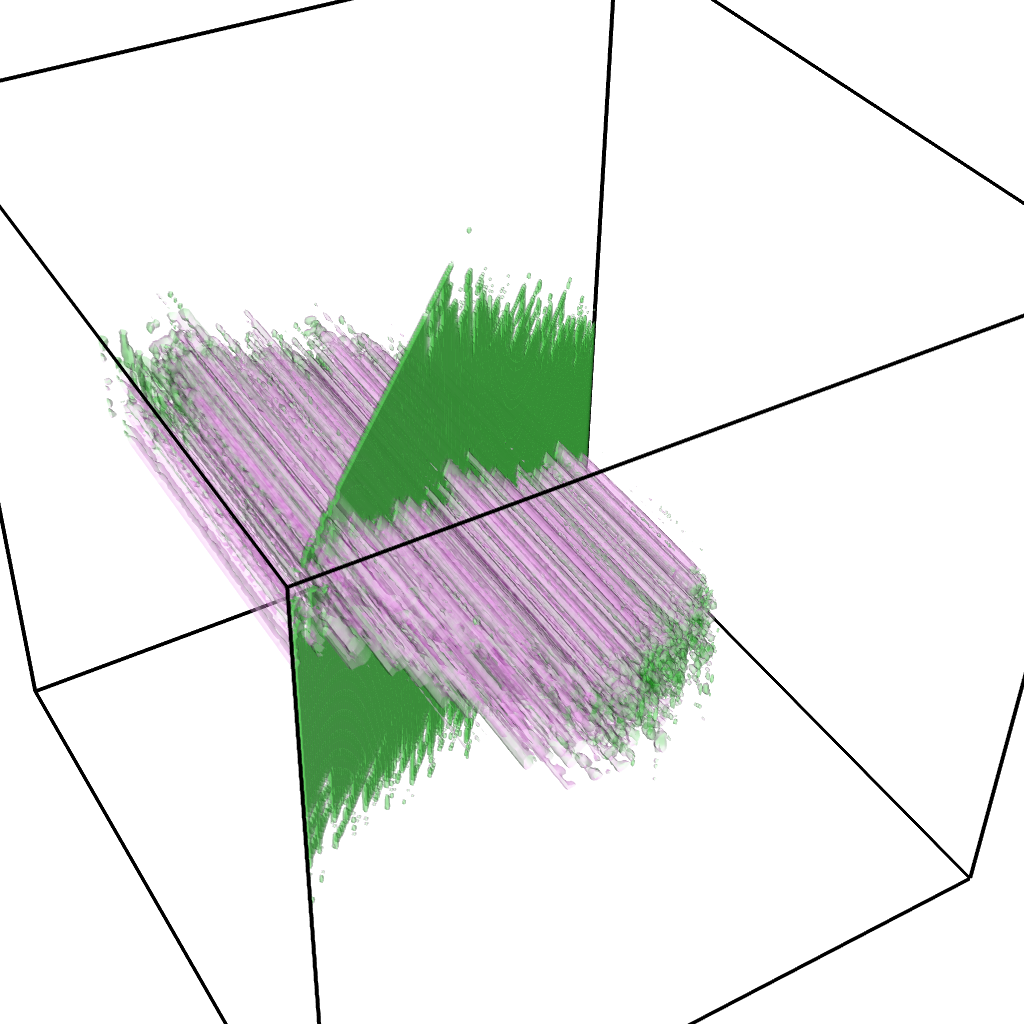
\includegraphics[width=1.5in,trim={6cm 6cm 6cm 6cm},clip]{y_15_tube_5_36.png}} 
\fbox{ 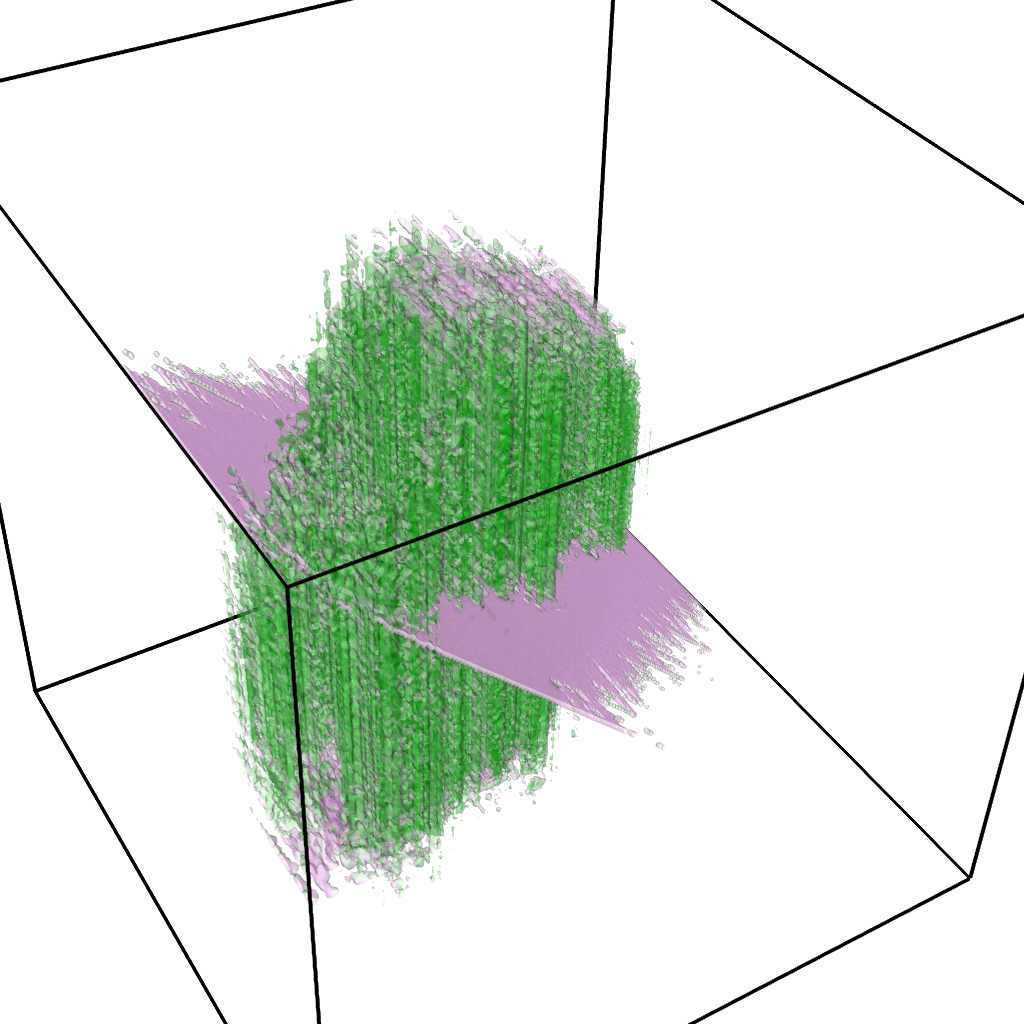
\includegraphics[width=1.5in,trim={6cm 6cm 6cm 6cm},clip]{z_15_tube_5_36.png}}
\end{figure}


\begin{figure}[h]
  \caption{equation...}
\fbox{ 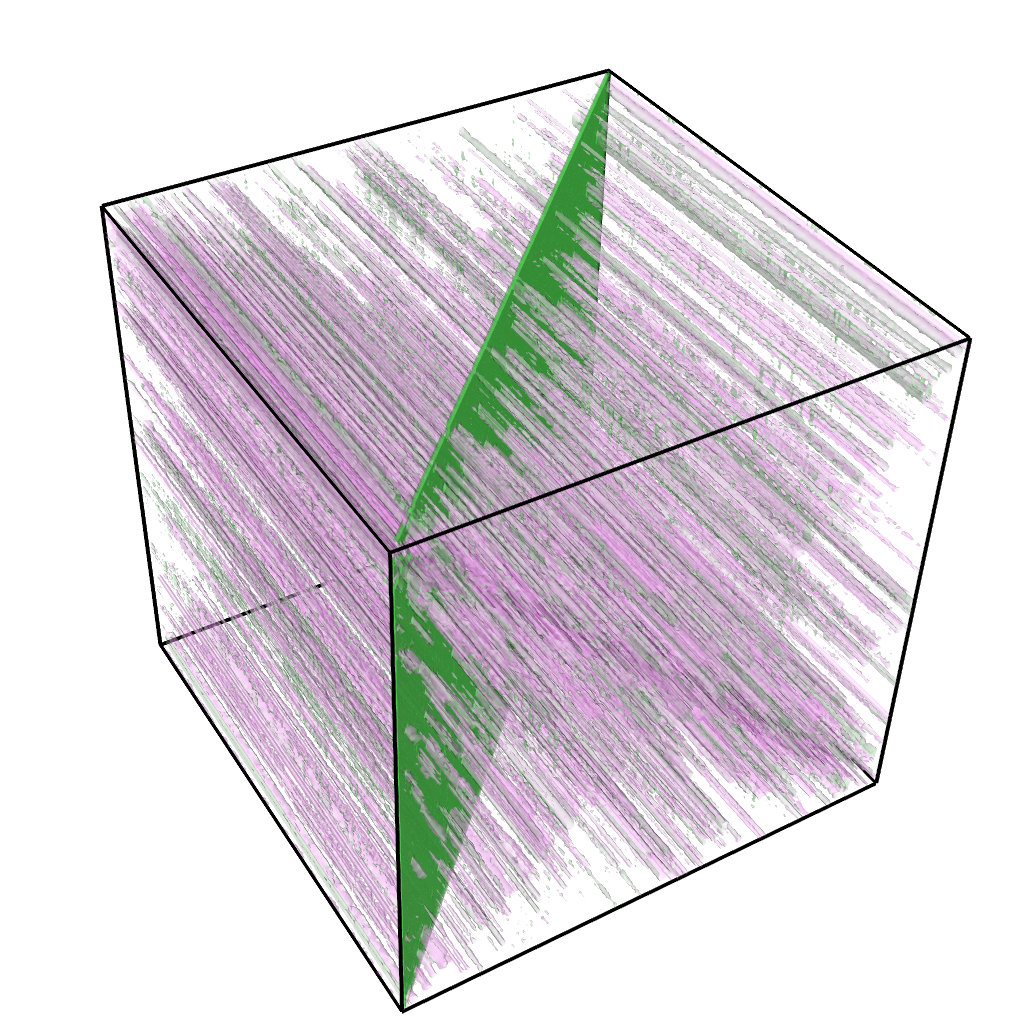
\includegraphics[width=1.5in,trim={6cm 6cm 6cm 6cm},clip]{y_15_water.png}} 
\fbox{ 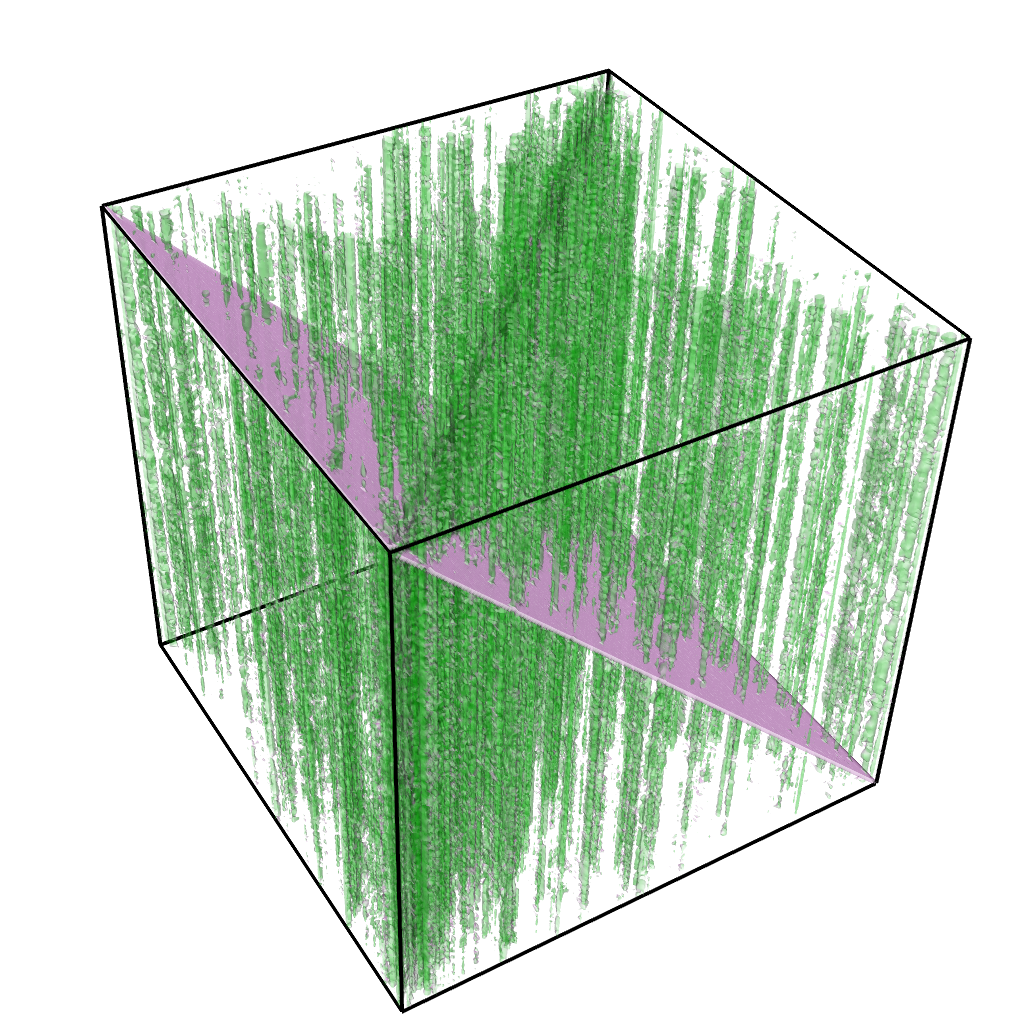
\includegraphics[width=1.5in,trim={6cm 6cm 6cm 6cm},clip]{z_15_water.png}}
\end{figure}

\begin{figure}[h]
  \caption{equation...}
%%\fbox{ \includegraphics[width=1.5in,trim={6cm 6cm 6cm 6cm},clip]{y_water_to_duals.png}} 
%%\fbox{ \includegraphics[width=1.5in,trim={6cm 6cm 6cm 6cm},clip]{z_water_to_duals.png}}
%\fbox{ \includegraphics[width=1.5in,trim={6cm 6cm 6cm 6cm},clip]{y_water_to_duals.png}} 
\fbox{ \includegraphics[width=3in,trim={8cm 0.1cm 8cm 0.1cm},clip]{z_water_to_duals_scn1.png}}
\end{figure}





\subsection{Comments}

\subsection{Found Contraction}

\subsection{Comments}
Pictures of the spamm structure

\section{Conclusion}

%%eg vs row-col picture.  Example of exact exchange w/DBSR 

\bibliography{MatrixFunctions}

\end{document}
